\begin{figure}
\begin{tabular}{@{}c@{}c@{}}
\hspace{10px}
\begin{subfigure}[b]{0.48\textwidth}
\begin{center}
\begin{allLangEnvFoot}
~{\scriptsize \textcolor{mygray}{S0:}}~ i32 sum_list (List l) {
~{\scriptsize \textcolor{mygray}{S1:}}~   i32 sum $\coloneqq$ ${\tt 0_{i32}}$;
~{\scriptsize \textcolor{mygray}{S2:}}~   while $\neg$(l is LNil):
~{\scriptsize \textcolor{mygray}{S3:}}~     // (l is LCons);
~{\scriptsize \textcolor{mygray}{S4:}}~     sum $\coloneqq$ sum + l.val;
~{\scriptsize \textcolor{mygray}{S5:}}~     l   $\coloneqq$ l.next;
~{\scriptsize \textcolor{mygray}{S6:}}~   return sum;
~{\scriptsize \textcolor{mygray}{SE:}}~ }
\end{allLangEnvFoot}
\end{center}
\caption{\label{figr:llTraverseSpecIR}(Abstracted) Spec IR}
\end{subfigure}%
&
\hspace{10px}
\begin{subfigure}[b]{0.52\textwidth}
\begin{center}
\begin{allLangEnvFoot}
~{\scriptsize \textcolor{mygray}{C0:}}~ i32 sum_list (i32 l) {
~{\scriptsize \textcolor{mygray}{C1:}}~   i32 sum $\coloneqq$ ${\tt 0_{i32}}$;
~{\scriptsize \textcolor{mygray}{C2:}}~   while ${\tt l \neq 0_{i32}}$:
~{\scriptsize \textcolor{mygray}{C3:}}~     sum $\coloneqq$ sum + $\structPointer{\tt l}{\mem{}}{lnode}{val}$;
~{\scriptsize \textcolor{mygray}{C4:}}~     l   $\coloneqq$ $\structPointer{\tt l}{\mem{}}{lnode}{next}$;
~{\scriptsize \textcolor{mygray}{C5:}}~   return sum;
~{\scriptsize \textcolor{mygray}{CE:}}~ }
\end{allLangEnvFoot}
\end{center}
\vspace{7px}
\caption{\label{figr:llTraverseCIR}(Abstracted) C IR}
\end{subfigure}%
\\
\begin{subfigure}[b]{0.48\textwidth}
\begin{center}
{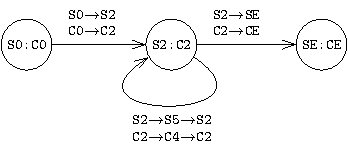
\includegraphics[scale=1.25]{chapters/figures/figSumListProductCfg.pdf}}
\end{center}
\caption{\label{figr:llTraverseProduct}Product-CFG between IRs \\ in \cref{figr:llTraverseSpecIR,figr:llTraverseCIR}}
\end{subfigure}%
&
\begin{subfigure}[b]{0.52\textwidth}
\begin{center}
\begin{footnotesize}
\begin{tabular}{cl}
\toprule
{\bf PC-Pair} & \multicolumn{1}{c} {\bf Invariants} \\
\toprule
(\scpc{0}{0}) & $\circled{P}\  \sv{l} \indEq{} \lifted{list}{\mem{}}{lnode}{\cv{l}}$ \\
\midrule
\multirow{2}{*}{(\scpc{2}{2})} & $\circled{\scriptsize I1}\  \sv{l} \indEq{} \lifted{list}{\mem{}}{lnode}{\cv{l}}$ \\ &
$\circled{\scriptsize I2}\  \sv{sum} = \cv{sum}$ \\
\midrule
(\scpc{E}{E}) & $\circled{\scriptsize E}\  \sv{ret} = \cv{ret}$ \\
\bottomrule
\end{tabular}
\end{footnotesize}
\end{center}
\caption{\label{figr:llTraverseProductInv}Node invariants for product-CFG in \cref{figr:llTraverseProduct}}
\end{subfigure}%
\\
\end{tabular}
\caption{\label{figr:llTraverseProductCFGInvs}\Cref{figr:llTraverseSpecIR,figr:llTraverseCIR} shows the IRs for the \SpecL{} and C {\tt sum\_list} procedures in \cref{fig:llTraverseSpec,fig:llTraverseC} respectively.
Product-CFG between the IRs in \cref{figr:llTraverseSpecIR,figr:llTraverseCIR} is shown in \cref{figr:llTraverseProduct}.
\Cref{fig:llTraverseProductInv} contains the corresponding node invariants for the product-CFG.}
\end{figure}
